\chapter{Site}

\begin{figure}[ht]
  \centering
  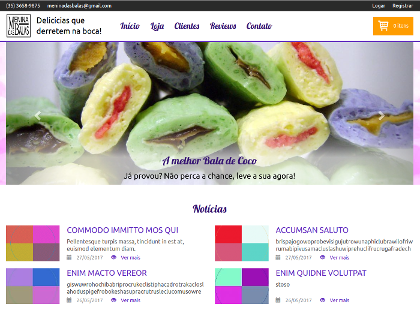
\includegraphics{site-1}
  \caption{Parte superior da página principal.}
  \label{site-1}
\end{figure}

\begin{figure}[ht]
  \centering
  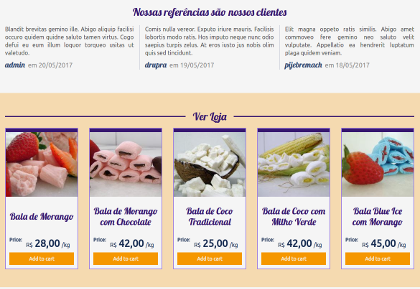
\includegraphics{site-2}
  \caption{Vitrine de produtos da página principal.}
  \label{site-2}
\end{figure}

\begin{figure}[ht]
  \centering
  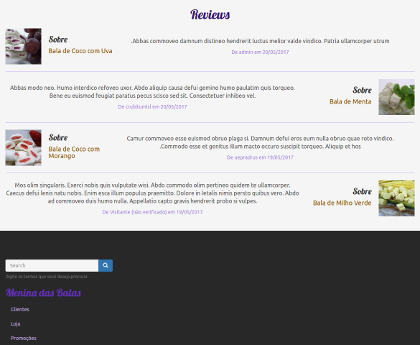
\includegraphics{site-3}
  \caption{Parte de baixo da página principal.}
  \label{site-3}
\end{figure}

\begin{figure}[ht]
  \centering
  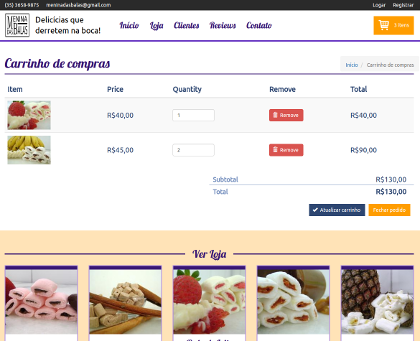
\includegraphics{site-4}
  \caption{Página do carrinho de compras com produtos.}
  \label{site-4}
\end{figure}
